\subsection{Fixed External Confirmation: Joint Increment Fails}
\label{sec:external}
After model and configuration selection on nuScenes development data, we evaluated five fixed methods on 20 independent AV2 logs, retaining all 936 actors: 878 build-ready, 58 missing-input, and 119 without owned heldout returns. The cohort includes 221 actors moving faster than 2\,m/s, 108 with unknown motion, and 556 with fewer than 100 build points. This is cross-dataset confirmation, not an untouched in-distribution nuScenes test. All methods use the already constructed cohort, calibration, known trajectories and fixed build-only metric alignment. There is no optimizer update, target-dependent calibration, new candidate, or selection using AV2 quality.

\begin{table*}[t]
\centering\small\begin{tabular}{lrrrrrr}
\toprule Method & Hit $\uparrow$ & Early $\downarrow$ & Miss $\downarrow$ & Free $\downarrow$ & Distance $\downarrow$ & Recall $\uparrow$ \\
\midrule
Joint r7 & 36.364 & 31.245 & 14.092 & 0.988 & 0.122 & 82.477 \\
LiDAR r6 & 39.306 & 25.881 & 15.055 & 0.662 & 0.109 & 84.898 \\
Narrow R8 & 38.093 & 10.012 & 42.661 & 0.117 & 0.126 & 82.069 \\
Native fusion & 28.090 & 10.868 & 55.552 & 0.345 & 0.146 & 79.093 \\
LiDAR PCA & 30.219 & 5.501 & 61.919 & 0.098 & 0.172 & 75.933 \\
\bottomrule\end{tabular}

\caption{Final fixed AV2 actor confirmation, 20 equally weighted logs. Hit/early/miss/recall are percentages; free and distance are meters. All 936 actor entries remain in accounting, including missing inputs and undefined owned-return cases. Distance is directed and conditional, not dense ground-truth Chamfer. Joint r7 and LiDAR r6 share the surface and physical objective; the joint pathway also changes native seeds, DPT features and build-depth auxiliary supervision.}
\label{tab:external}
\end{table*}
\begin{table}[t]
\centering\scriptsize\begin{tabular}{lrrr}
\toprule Metric & $\Delta$ & 95\% log interval & Better \\
\midrule
Hit (pp) & -2.942 & $[-4.799,-1.011]$ & 5/20 \\
Early (pp) & +5.364 & $[+3.504,+7.153]$ & 2/20 \\
Miss (pp) & -0.962 & $[-1.937,+0.058]$ & 13/20 \\
Free (m) & +0.326 & $[+0.254,+0.400]$ & 0/20 \\
Distance (m) & +0.013 & $[+0.006,+0.021]$ & 5/20 \\
Recall (pp) & -2.420 & $[-4.078,-0.772]$ & 6/20 \\
\bottomrule\end{tabular}

\caption{External Joint r7 minus matched LiDAR r6. Five adverse intervals exclude zero. The slight missing reduction is uncertain.}
\label{tab:external-pair}
\end{table}
The development improvement does not survive this confirmation. Against r6, joint r7 loses 2.942\,pp correct hits and 2.420\,pp recall, while early increases 5.364\,pp, free intrusion increases 0.3260\,m, and target-to-surface distance increases 0.01326\,m. All five paired 95\% log bootstrap intervals exclude zero in the adverse direction. Free intrusion worsens in all 20 logs. Missing changes $-0.962$\,pp with interval $[-1.937,0.058]$; this does not establish improvement or equivalence. The final joint pathway therefore \emph{fails independent confirmation of a generalizable geometry-and-physics increment}. We retain its supported development gains instead of rewriting them as an absence of learning.

Compared with narrow R8, joint reduces missing by 28.569\,pp but adds 21.232\,pp early and 0.8707\,m free intrusion; all three intervals exclude zero. Hit, distance and recall differences against R8 have intervals crossing zero. Joint improves hit and measured coverage over native fusion and PCA, but both comparisons also increase early and free intrusion. Selecting only missing rate or a weaker baseline would misrepresent this trade-off.

\begin{figure*}[t]
\centering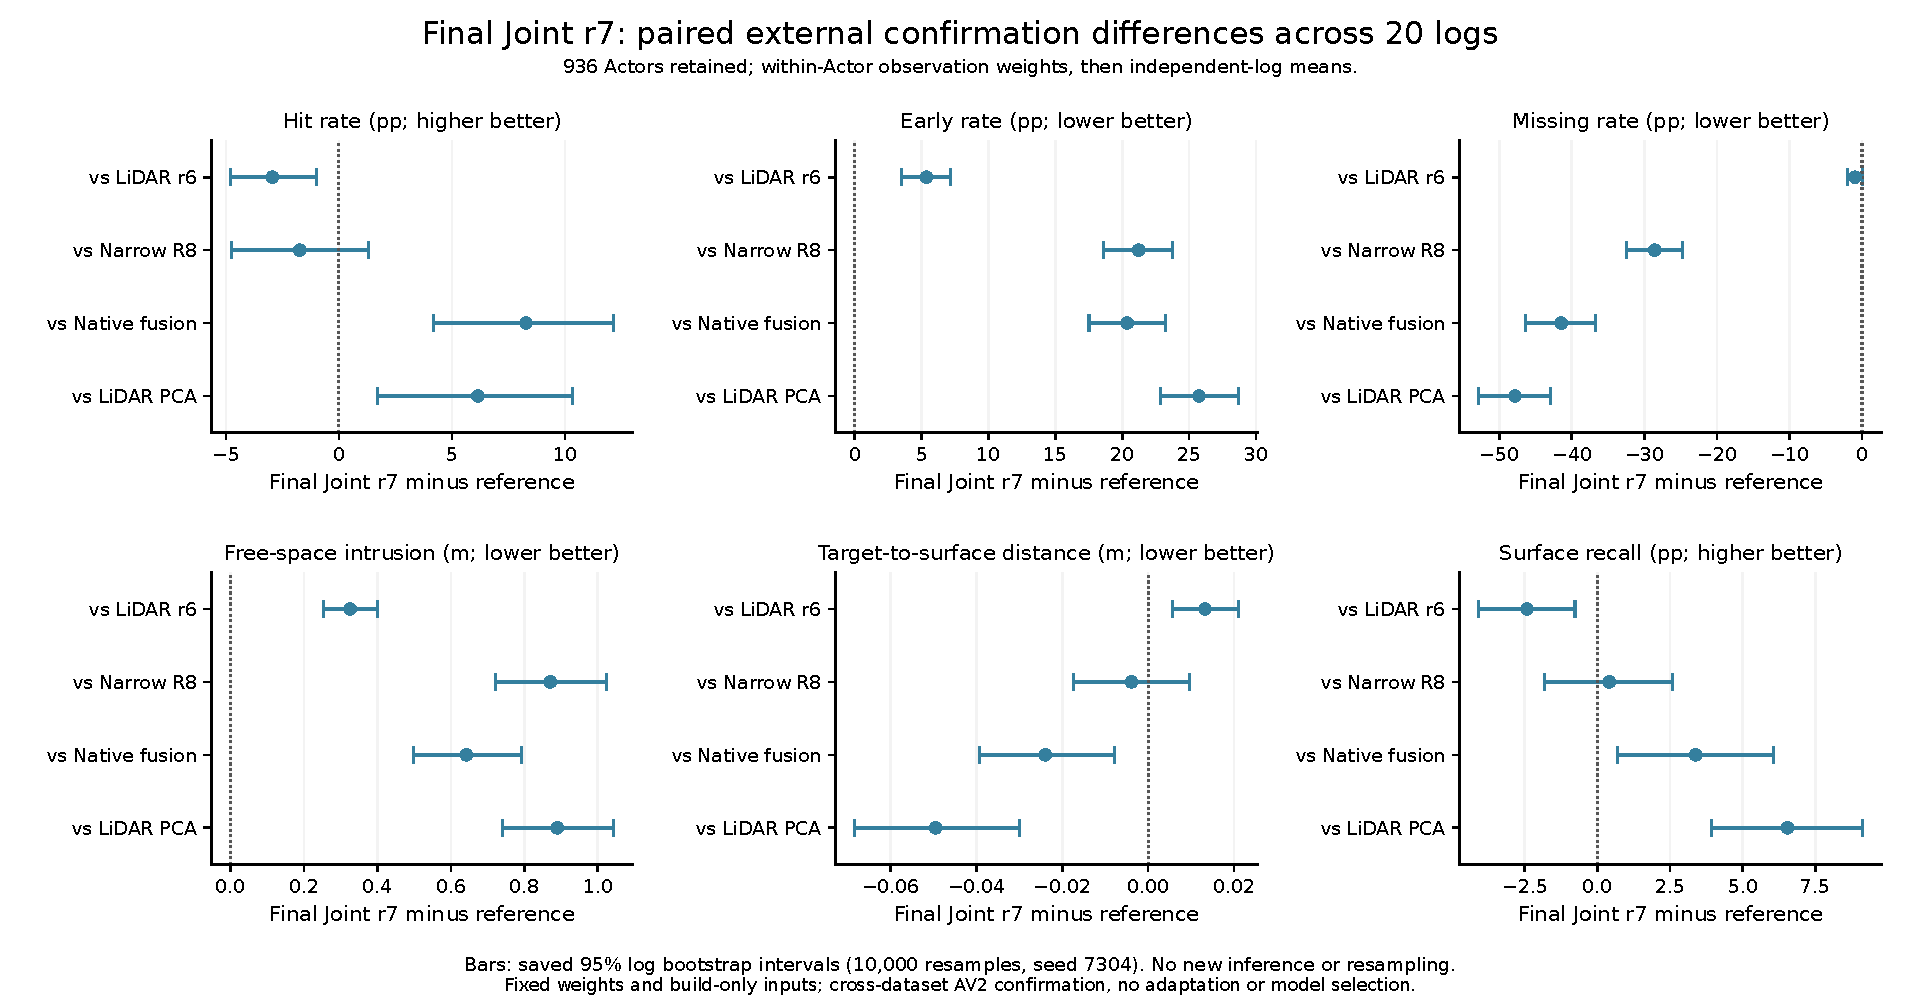
\includegraphics[width=\textwidth]{figures/v73/external_pairs.pdf}
\caption{All four fixed external comparisons from the saved log bootstrap, with no new resampling or model selection. The matched r6 comparison is primary. More coverage relative to narrow or fused baselines does not imply a more physically consistent surface.}
\label{fig:external}
\end{figure*}
The fixed inference runs take 1239.62, 282.67, 1729.72, 1700.97 and 1457.57 seconds for joint, r6, R8, native fusion and PCA respectively, including loading and evaluation. Peak CUDA allocations are 5.439, 0.056, 0.056, 1.302 and 0.022\,GiB; joint/native peak process RSS is 44.07/44.77\,GiB. All finish with zero optimization updates. These measured costs do not establish equal throughput at different surface densities.

The observed failure is a cross-domain reversal and a surface/free-space conflict. Development forensics already show that regular supported patches can extend into the wrong first-surface location. Dataset and camera-system shifts, residual alignment error, local correspondence contamination and support-domain extent are plausible contributors, not isolated causes. This whole-pathway comparison cannot identify a pure visual-feature effect, and it does not show that all visual foundations are ineffective. Neither missing resources nor an absent DPT gradient explains the completed experiment. The learned support-boundary and orthogonal-update proposals remain untested follow-up ideas, not retroactive components of r7 or a reason to continue this closed experimental sequence.
